% #############################################################################
% This is Chapter 4
% !TEX root = ../main.tex
% #############################################################################
% Change the Name of the Chapter i the following line
\fancychapter{Conducted Numerical Simulations}
% \cleardoublepage
% The following line allows to ref this chapter
\label{chap:implement}

% Aliquam aliquet, est a ullamcorper condimentum, tellus nulla fringilla elit, a iaculis nulla turpis sed wisi. Fusce volutpat. Etiam sodales ante id nunc. Proin ornare dignissim lacus. Nunc porttitor nunc a sem. Sed sollicitudin velit eu magna. Aliquam erat volutpat. Vivamus ornare est non wisi. Proin vel quam. Vivamus egestas. Nunc tempor diam vehicula mauris. Nullam sapien eros, facilisis vel, eleifend non, auctor dapibus, pede. 
% % #############################################################################
% \section{Poisson Equation using MFS-B}
% Suspendisse vestibulum dignissim quam. Integer vel augue. Phasellus nulla purus, interdum ac, venenatis non, varius rutrum, leo. Pellentesque habitant morbi tristique senectus et netus et malesuada fames ac turpis egestas. Duis a eros. Class aptent taciti sociosqu ad litora torquent per conubia nostra, per inceptos hymenaeos. Fusce magna mi, porttitor quis, convallis eget, sodales ac, urna. Phasellus luctus venenatis magna. Vivamus eget lacus. Nunc tincidunt convallis tortor. Duis eros mi, dictum vel, fringilla sit amet, fermentum id, sem. Phasellus nunc enim, faucibus ut, laoreet in, consequat id, metus. Vivamus dignissim. Cras lobortis tempor velit. Phasellus nec diam ac nisl lacinia tristique. Nullam nec metus id mi dictum dignissim. Nullam quis wisi non sem lobortis condimentum. Phasellus pulvinar, nulla non aliquam eleifend, tortor wisi scelerisque felis, in sollicitudin arcu ante lacinia leo.:

% \begin{itemize}
% \item{Technology Research and Related Works}
% \item{Requirements Gathering and Study}
% \item{Design of the Architecture}
% \item{Implementation Process}
% \item{Testing and Functional Validation}
% \end{itemize}

% Pellentesque nibh felis, eleifend id, commodo in, interdum vitae, leo. Praesent eu elit. Ut eu ligula. Class aptent taciti sociosqu ad litora torquent per conubia nostra, per inceptos hymenaeos. Maecenas elementum augue nec nisl. Proin auctor lorem at nibh. Curabitur nulla purus, feugiat id, elementum in, lobortis quis, pede. Vivamus sodales adipiscing sapien. Vestibulum posuere nulla eget wisi. Integer volutpat ligula eget enim. Suspendisse vitae arcu. Quisque pellentesque. Nullam consequat, sem vitae rhoncus tristique, mauris nulla fermentum est, bibendum ullamcorper sapien magna et quam. Sed dapibus vehicula odio. Proin bibendum gravida nisl. Fusce lorem. Phasellus sagittis, nulla in hendrerit laoreet, libero lacus feugiat urna, eget hendrerit pede magna vitae lorem. Praesent mauris.
% % #############################################################################
% \section{Poisson Equation using MFS-D}
% Cras sed ante. Phasellus in massa. Curabitur dolor eros, gravida et, hendrerit ac, cursus non, massa. Aliquam lorem. In hac habitasse platea dictumst. Cras eu mauris \Cref{time_control_algorithm}\todo[color=cyan!40, author=RC, fancyline]{Notice the reference to the Algorithm construct}{}. Quisque lacus. Donec ipsum. Nullam vitae sem at nunc pharetra ultricies. Vivamus elit eros, ullamcorper a, adipiscing sit amet, porttitor ut, nibh. 

% \begin{algorithm}[ht]
% \DontPrintSemicolon
% \Begin{
% $nextBitrate \longleftarrow nextDownloadLevel$\;
% $nextBitrate \longleftarrow GetNextBitrate()$\;
% $cpuLoad \longleftarrow GetCpuLoad()$\;
% $bitrateDelta \longleftarrow getBitrateDelta(currentBitrate, nextBitrate)$\;
% \BlankLine
% \If{$bitrateDelta > maxThreshold$}{
%      $SetBitrate(nextBitrate)$\;
%    }
% \BlankLine
%   \If{$minThreshold < bitrateDelta < maxThreshold$ {\bf and} $numAttemps < 2$}{ 
%        $numAttemps \longleftarrow numAttemps + 1$\;
%        }{
%        \uElseIf{$minThreshold < bitrateDelta < maxThreshold$ {\bf and} $numAttemps = 2$}{
%        $numAttemps \longleftarrow 0$\;
%        }
%        \Else{$SetBitrate(nextBitrate)$}
%       }
%   \If{$0 < bitrateDelta < minThreshold$ {\bf and} $numAttemps < 3$}{
%        $numAttemps \longleftarrow numAttemps + 1$\;
%        }{
%        \uElseIf{$0 < bitrateDelta < minThreshold$ {\bf and} $numAttemps = 3$}{
%        $SetBitrate(nextBitrate)$\;
%        }
%        }
% }
% \caption{Time Control Strategy}
% \label{time_control_algorithm}
% \end{algorithm}


% Maecenas adipiscing mollis massa. Nunc ut dui eget nulla venenatis aliquet. Sed luctus posuere justo. Cras vehicula varius turpis. Vivamus eros metus, tristique sit amet, molestie dignissim, malesuada et, urna..
% % #############################################################################
% \section{Helmholtz Equation using MFS-B}
% Cras sed ante. Phasellus in massa. Curabitur dolor eros, gravida et, hendrerit ac, cursus non, massa. Aliquam lorem. In hac habitasse platea dictumst. Cras eu mauris. Quisque lacus. Donec ipsum. Nullam vitae sem at nunc pharetra ultricies. 

% Vivamus elit eros, ullamcorper a, adipiscing sit amet, porttitor ut, nibh. Maecenas adipiscing mollis massa. Nunc ut dui eget nulla venenatis aliquet. Sed luctus posuere justo. Cras vehicula varius turpis. Vivamus eros metus, tristique sit amet, molestie dignissim, malesuada et, urna.

% Quisque lacus. Donec ipsum. Nullam vitae sem at nunc pharetra ultricies. Cras vehicula varius turpis.



% \begin{minipage}[c]{1.0\textwidth}
% %\begin{center}
% \centering
% \begin{lstlisting}[language = C++, numbers = none, escapechar = !,
%     basicstyle = \ttfamily\bfseries, linewidth = .6\linewidth, frame=tb, caption={A listing with a Tikz picture overlayed}, captionpos=b, label=tikzlist] 
%  int!
%    \tikz[remember picture] \node [] (a) {};
%  !puissance!
%    \tikz[remember picture] \node [] (b) {};
%  !(int x,!
%    \tikz[remember picture] \node [] (c){};
%  !int n) { 

%      int i, p = 1; !\tikz[remember picture] \node [] (d){};!           

%      for (i = 1; i <= n; i++) 
%        p = p * x; !\tikz[remember picture] \node [inner xsep = 40pt] (e){};! 

%      return p; !
%        \tikz[remember picture] \node [] (f){};!  
%  }
% \end{lstlisting}

% \begin{tikzpicture}[remember picture, overlay,
%     every edge/.append style = { ->, thick, >=stealth,
%                                   darkgray, dashed, line width = 1pt },
%     every node/.append style = { align = center, minimum height = 10pt,
%                                  font = \bfseries, fill= green!20},
%                   text width = 2.5cm ]
%   \node [above left = .75cm and -.75 cm of a,text width = 2.2cm]
%                              (A) {return value type};
%   \node [right = 0.25cm of A, text width = 1.9cm]
%                              (B) {function name};
%   \node [right = 0.5cm of B] (C) {list of formal parameters};
%   \node [right = 4.cm of d]  (D) {local variables declaration};
%   \node [right = 2.cm of e]  (E) {instructions};
%   \node [right = 5.cm of f]  (F) {instruction \texttt{\bfseries return}};  
%   \draw (A.south) + (0, 0) coordinate(x1) edge (x1|-a.north);
%   \draw (B.south) + (0, 0) coordinate(x2) edge (x2|-b.north);
%   \draw (C.south) + (0, 0) coordinate(x3) edge (x3|-c.north);
%   \draw (D.west) edge (d.east) ;
%   \draw (E.west) edge (e.east) ;  
%   \draw (F.west) edge (f.east) ;
% \end{tikzpicture}
% %\end{center}
% \end{minipage}

% \textcolor{violet}{And here another method (\Cref{tikzlist}) for mixing (overlay) a picture with a listing of code.}
% % #############################################################################
% \subsection{User Interface}
% Donec semper turpis sed diam. Sed consequat ligula nec tortor. Integer eget sem. Ut vitae enim eu est vehicula gravida. Morbi ipsum ipsum, porta nec, tempor id, auctor vitae, purus. Pellentesque neque. Nulla luctus erat vitae libero. Integer nec enim. Phasellus aliquam enim et tortor. Quisque aliquet, quam elementum condimentum feugiat, tellus odio consectetuer wisi, vel nonummy sem neque in elit. Curabitur eleifend wisi iaculis ipsum. Pellentesque habitant morbi tristique senectus et netus et malesuada fames ac turpis egestas. In non velit non ligula laoreet ultrices. Praesent ultricies facilisis nisl. Vivamus luctus elit sit amet mi. Phasellus pellentesque, erat eget elementum volutpat, dolor nisl porta neque, vitae sodales ipsum nibh in ligula. Maecenas mattis pulvinar diam. Curabitur sed leo..

% Cras eu mauris. Quisque lacus. Donec ipsum. Nullam vitae sem at nunc pharetra ultricies. Vivamus elit eros, ullamcorper a, adipiscing sit amet, porttitor ut, nibh. Maecenas adipiscing mollis massa. Nunc ut dui eget nulla venenatis aliquet. Sed luctus posuere justo. Cras vehicula varius turpis. 
% % #############################################################################
% \subsection{Vivamus luctus elit sit amet mi}
% Nulla facilisi. In vel sem. Morbi id urna in diam dignissim feugiat. Proin molestie tortor eu velit. Aliquam erat volutpat. Nullam ultrices, diam tempus vulputate egestas, eros pede varius leo, sed imperdiet lectus est ornare odio. Lorem ipsum dolor sit amet, consectetuer adipiscing elit. Proin consectetuer velit in dui. Phasellus wisi purus, interdum vitae, rutrum accumsan, viverra in, velit. Sed enim risus, congue non, tristique in, commodo eu, metus. Aenean tortor mi, imperdiet id, gravida eu, posuere eu, felis. 

% Mauris sollicitudin, turpis in hendrerit sodales, lectus ipsum pellentesque ligula, sit amet scelerisque urna nibh ut arcu. Aliquam in lacus. 

% \Cref{fig:ui_playout,fig:ui_loading}\todo[color=cyan!40, author=RC, fancyline]{A figure with Subfigures}{} proin at eros non eros adipiscing mollis.

% \begin{figure}[htbp]
% 	\centering
% 	\subfigure[Media Loading Window]{\label{fig:ui_loading} 		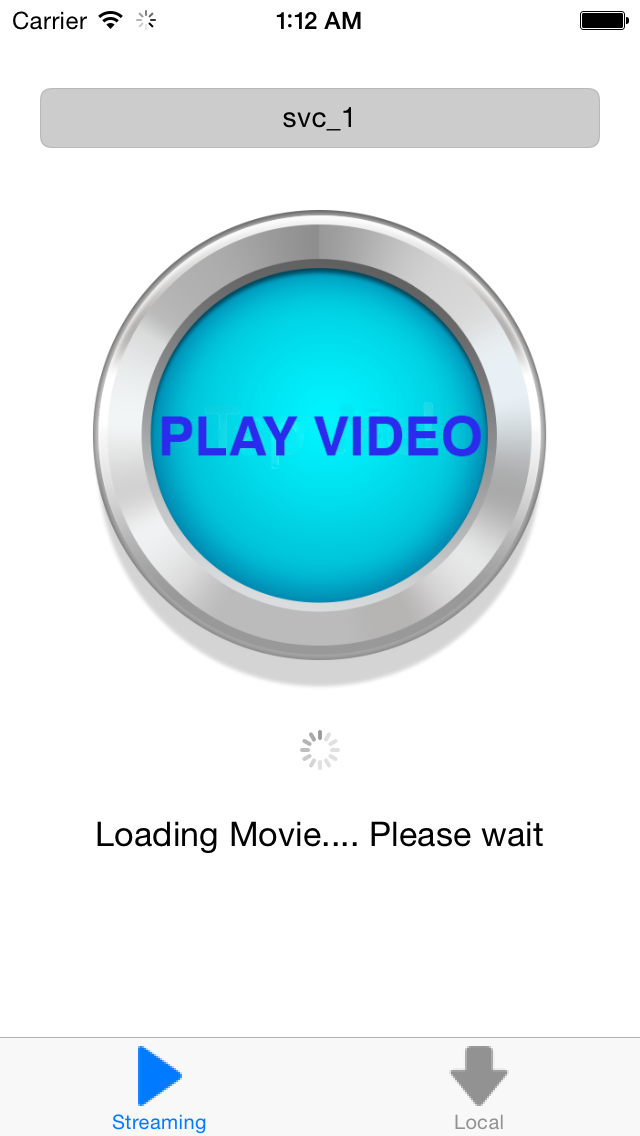
\includegraphics[width=0.3\textwidth]{./Images/ui_loading}} \qquad
% 	\subfigure[Play-out Session UI]{\label{fig:ui_playout}
% 		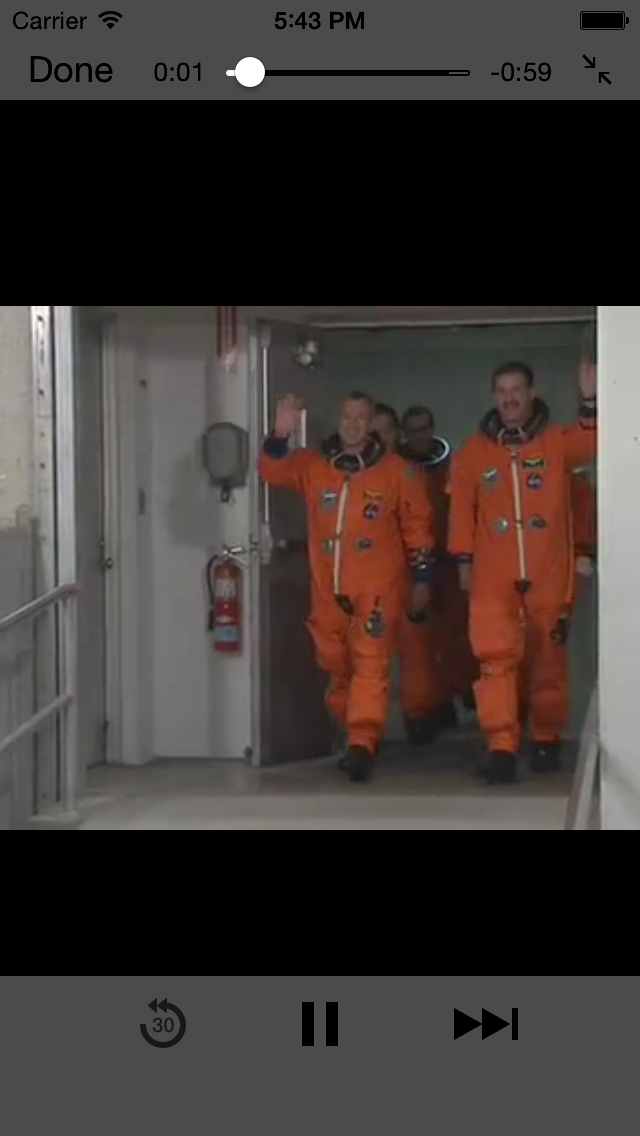
\includegraphics[width=0.3\textwidth]{./Images/ui_playout}}
% 	\caption{Complete User Interface}
% 	\label{fig:user_interface}
% \end{figure}

% Vestibulum ante ipsum primis in \ac{UI} faucibus orci luctus et ultrices posuere cubilia Curae; Nulla placerat aliquam wisi. Mauris viverra odio. Quisque fermentum pulvinar odio. Proin posuere est vitae ligula. Etiam euismod. Cras a eros.



